\section{Experimental Evaluation}
\label{sec:exp}

{\bf Experimental environment.} All experiments in this section were
conducted on an 8-slave elastic cloud cluster using Linux Ubuntu 14.04
and Spark v1.4.  Each node had 4 cores and 16 GB of memory.  Spark
Standalone cluster manager and Hadoop 2.6 were used.

Because Spark is a lazy evaluation system, a \insql{materialize}
operation was appended to the end of each query, which consisted of
the count of nodes and edges.  In cases where the goal was to evaluate
a specific operation in isolation, we used warm start which consisted
of materializing the graph upon load.  Each experiment was conducted 3
times, we report the average running time. \eat{ and the measure of
variability.}

{\bf Data and evaluation methods.}  We evaluate performance of our
framework on two real open-source datasets:

\begin{enumerate}%[leftmargin=*]

\item DBLP\footnote{\url{dblp.uni-trier.de/xml}} contains
  co-authorship information from 1936 \linebreak through 2015, with over 1.5
  million author nodes and over 6 million undirected co-authorship
  edges.  Total data size: 250 MB.

\item nGrams\footnote{\url{storage.googleapis.com/books/ngrams/books/datasetsv2.html}}
  contains word co-occurrence information from 1520 through 2008, with
  over 1.5 million word nodes and over 65 million undirected
  co-occurrence edges.  Total data size: 40 GB.
\eat{
\item
  DELIS\footnote{\url{law.di.unimi.it/webdata/uk-union-2006-06-2007-05}}
  contains monthly snapshots of a portion of the Web graph focusing on
  the .uk domains from 05/2006 through 05/2007, with a total of over
  133 million nodes and over 5.5 billion directed edges\cite{BSVLTAG}.
  Data size: 1 TB.
}
\end{enumerate}

These datasets are not large by industry standards, but
the nGrams set is of comparable size to the LiveJournal dataset
in~\cite{Xin2013} and is commesurate with our cluster size.  We plan to
carry out further experiments with a larger
DELIS\footnote{\url{law.di.unimi.it/webdata/uk-union-2006-06-2007-05}}
dataset as we grow the cluster in the near future.

\subsection{Number of partitions}

\begin{figure*}[th!]
\centering
\begin{minipage}{3.3in}
  \centering
  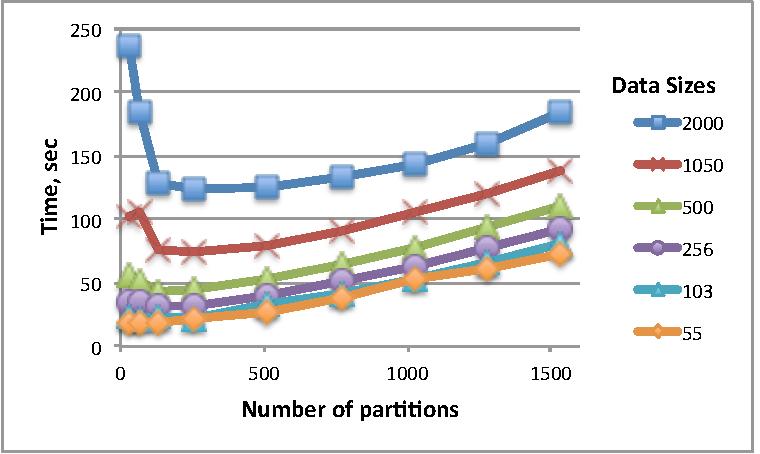
\includegraphics[width=3in]{figs/numparts.pdf}
  \caption{The number of partitions trend for different data sizes.}
  \label{fig:numparts}
\end{minipage}
\begin{minipage}{3.3in}
  \centering
  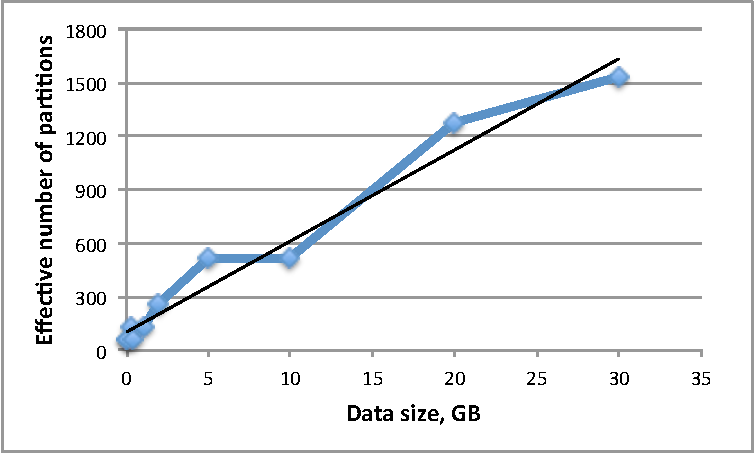
\includegraphics[width=3in]{figs/partsfit.pdf}
  \caption{Relationship between data size and the effective number of
  partitions.}
  \label{fig:partsfit}
\end{minipage}
\end{figure*}

In Spark applications, one of the most influential performance drivers
is the choice of the number of partitions.  The default number of
partitions, based on the Hadoop block size, used to read the graphs in
practice proved insufficient.  We extended GraphX for parallel reading
of multiple files with a custom number of partitions.  For all
experiments a dynamic data size-based partition number estimator was
used based on the tuning experiment.

To tune the estimator, we ran a simple \insql{TSelect} query with each
data structure, varying the number of partitions on load for a range
of data sizes.  In each data structure, we observe the same trend --
as the number of partitions is increased for a given data size, the
system performance quickly improves, but then starts to deteriorate
(Figure~\ref{fig:numparts}).  This trend can be observed in all data
structures.  As can be seen in Figure~\ref{fig:partsfit}, there is
roughly a linear relationship between the data size and the optimal
number of partitions, which allowed us to fit a linear function and
use it in all subsequent experiments.

\subsection{Data loading}

To understand how different data structures perform as a function of
data size, we ran a simple TSelect query:

\begin{small}
\begin{verbatim}
      TSelect V; E
      From    ngrams
      TWhere  Start >= x and End <= y
\end{verbatim}
\end{small}

\noindent where \insql{x} and \insql{y} parameters were varied to
achieve approximate desired data sizes for edge files.  Our file
format is a node file and an edge file per snapshot, with a node/edge
per line, respectively.  This format favors the SG data structure
because no data transformation, such as aggregation, is required.
This is substantiated experimentally, as can be seen in
Figure~\ref{fig:tselect}.  In the nGrams dataset, SG is the fastest
data structure for simple data loading, although all structures
exhibit a linear increase as a function of data size.  We observed the
same trend in both datasets and are not including the additional
graphs here. 

The significant influence of data format on data structure performance
has been shown previously~\cite{DBLP:journals/tos/MiaoHLWYZPCC15}.
Given the significant difference at size (3-5x) between SG and the
other data structures, an alternative file format for aggregated data
structures is warranted.  Because the load/materialize time varies so
significantly between different data structures, all subsequent
experiments are reported with a warm start, with application of a
desired partition strategy included during the loading process.

\begin{figure}[t!]
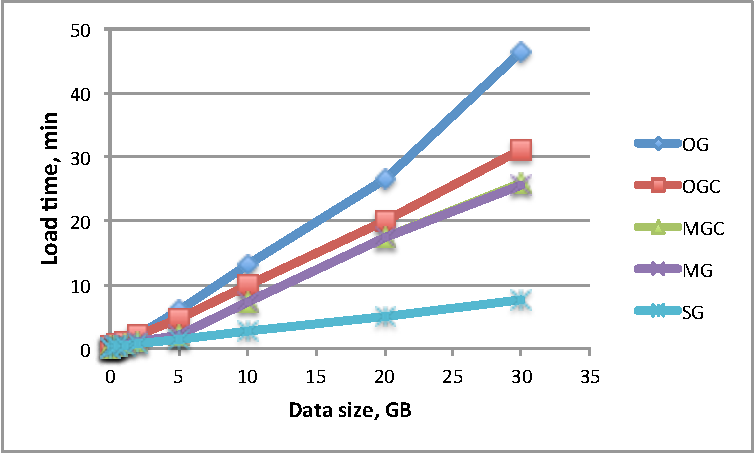
\includegraphics[width=3.2in]{figs/tselect.pdf}
\caption{Total load time as a function of data size in the nGrams
  dataset.}
\label{fig:tselect}
\end{figure}

\subsection{\insql{TSelect} with \insql{TGroup}}

To investigate the comparative performance of different data
structures and partition strategies on the TGroup operation, we used
the following query:

\begin{small}
\begin{verbatim}
      TSelect Any V[vid, any(word)];
              Any E[vid1, vid2, sum(cnt) as score]
      From    nGrams
      TWhere  Start >= x And End <= y
      TGroup  by 8 years
\end{verbatim}
\end{small}

We kept the aggregation time window constant (8 years) and varied the
total number of snapshots (indicated as \insql{x} and \insql{y}) in
powers of 2.  Each snapshot contained about 13 million edges.

Recollect that \insql{TGroup} requires a union and group by operation
in SG, combination of transform with filter and group by for MG, and
transform with filter for OG.  MGC, due its compactness, generally
outperforms MG and OGC -- OG, and here we include only the better
performing variant of each.  All data structures and partition
strategies show linear increase in Any-type aggregation time as the
number of snapshots grows.  As expected, because OGC is an already
aggregated data structure, it outperforms MGC and SGP for the
\insql{TGroup} operation by two orders of magnitude in the largest
size (Figure~\ref{fig:tgroupe}).

\begin{figure*}[t!]
\centering
\begin{minipage}{3.3in}
  \centering
  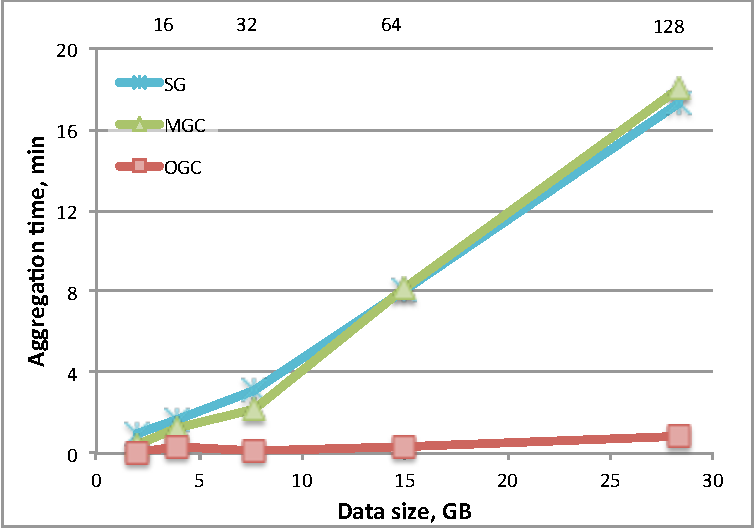
\includegraphics[width=3in]{figs/tgroupe_warm.pdf}
  \caption{\insql{TGroup} with Any after materialization.}
  \label{fig:tgroupe}
\end{minipage}
\begin{minipage}{3.3in}
  \centering
  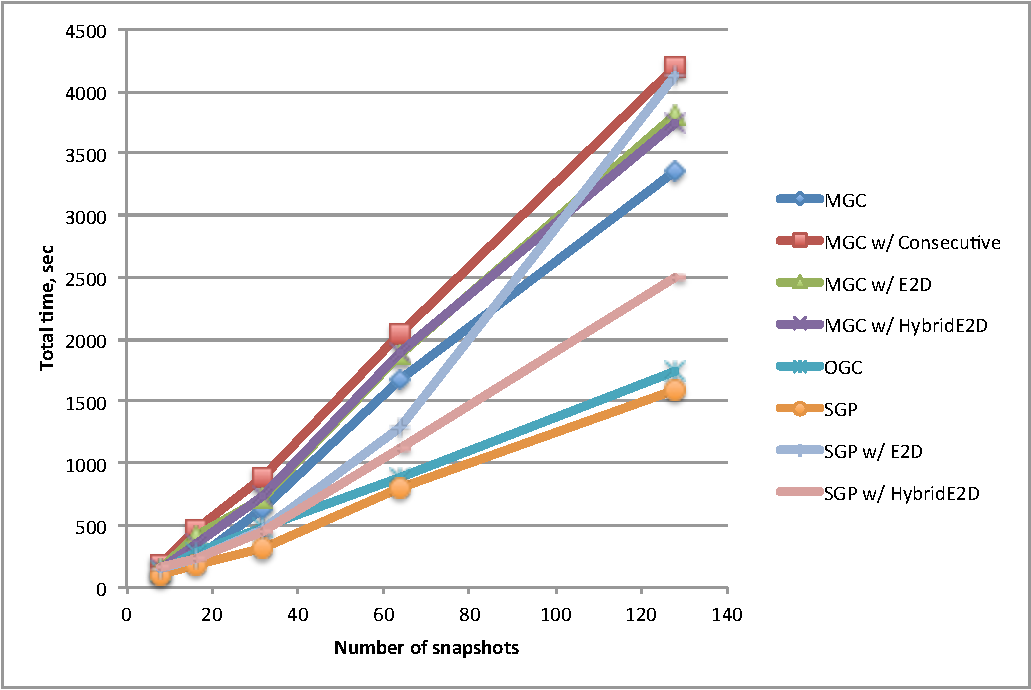
\includegraphics[width=3in]{figs/tgroupe_cold.pdf}
  \caption{\insql{TGroup} with Any with materialization.}
\label{fig:tgroupe_cold}
\end{minipage}
\end{figure*}

Note that partition strategies can improve performance for the MGC
data structure on this operation -- all outperform the default
partitioning case by 20\% or greater.  This can be explained by the
group by operation that is performed on the edges.  E2D always places
two edges with the same key in the same partition, which theoretically
leads to least cross-partition communication during aggregation.
Hybrid strategies use the aggregation window as the width of the run,
also placing the edges that are to be grouped in the same set of
partitions.  The difference between E2D and the hybrid strategies for
the MGC data structure are not statistically significant.
Partitioning of the SG is also beneficial, but the gains are smaller
than for the MGC.  We observed the same trend for the TGroup query
with All semantics -- see Appendix.

To demonstrate why we use warm start, consider
Figure~\ref{fig:tgroupe_cold}.  When we consider the total time for
the same query, including graph loading, partitioning, aggregation,
and materialization, the loading time dominates.  Based on this graph
in isolation, one can conclude that partitioning is not beneficial
(because it takes additional non-trivial time) and that SG is the most
effective data structure.  However, recal from experiment 1 that the
file format favors SG, and no conclusions should be drawn from cold
start total time alone.

\vera{If we get to run the version where we vary the aggregation
  window, include it here.}

\subsection{\insql{TAnd} with \insql{All}}

\insql{TAnd} is a binary operation, and thus co-partitioning of the
two evolving graphs should play a role in performance.  Similarly to
\insql{TGroup} above, we look at the warm start performance of each
data structure and partition strategy, using the following query:

\begin{small}
\begin{verbatim}
      TSelect All V[vid, max(word)];
              All E[vid1, vid2, max(cnt) as score]
      From    ( TSelect V; E
                From nGrams
                TWhere  Start >= x And End <= y )
              TAnd
              ( TSelect V; E
                From nGrams
                TWhere  Start >= n And End <= m )      
\end{verbatim}
\end{small}

We are selecting the two graphs from the same dataset and varying the
amount of temporal overlap (\insql{n - m}) between them to investigate
the worst-case performance.  This query is a good example where
pushing selection would lead to some performance improvement, since
only the \insql{n} to \insql{y} snapshots are relevant to the
operation.  In this experiment the query was not optimized in this
fashion and executed directly as specified.

\insql{TAnd} requires a join operation for each snapshot pair in SG,
and a single graph join in all other data structures.  As the temporal
overlap between the two graphs increases, we expect OGC to outperform
SG, and this can be shown experimentally (Figure~\ref{fig:tandall}).

\begin{figure}[t!]
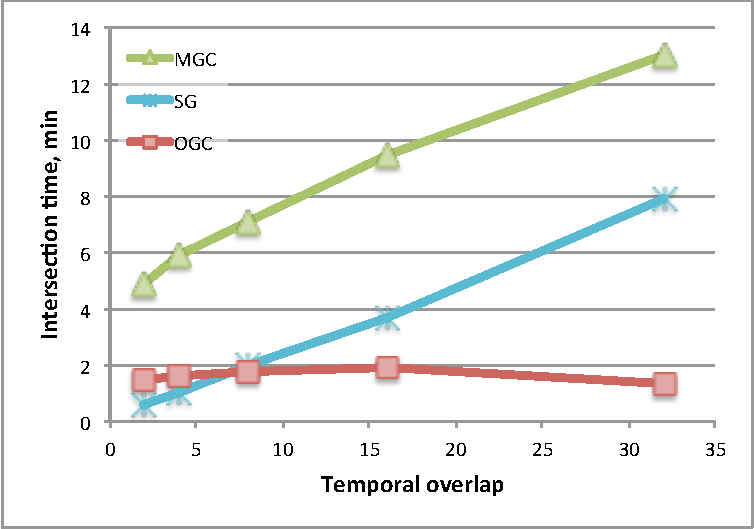
\includegraphics[width=3.2in]{figs/tand_all_warm.pdf}
\caption{As the temporal overlap increases, so does the TAnd time, for
  all data structures and partition strategies.  OG outperforms the
  other data structures.}
\label{fig:tandall}
\end{figure}

MORE HERE

\subsection{\insql{TSelect} with \insql{trend(pagerank())}}

